% Niveau :      PCSI - PC
% Discipline :  Elec
% Mots clés :   Elec, Ordre 2

\begin{exercise}{Tube fluorescent}{1}{Sup,Spé}
{\'Electrocinétique, Circuits d'ordre 2}{bermu}


Les tubes fluorescents sont un type particulier de lampes électriques qui produisent de la lumière grâce à une décharge électrique.

Ces tubes s'allument quand la tension à leur bornes dépasse une certaine tension d'allumage $U_a$. Un fois allumé, le tube s'éteint quand la tension descend en dessous de $U_e$, la tension d'extinction, comme l'illustre la figure ci-dessous.

\begin{figure}[H]
    \centering
    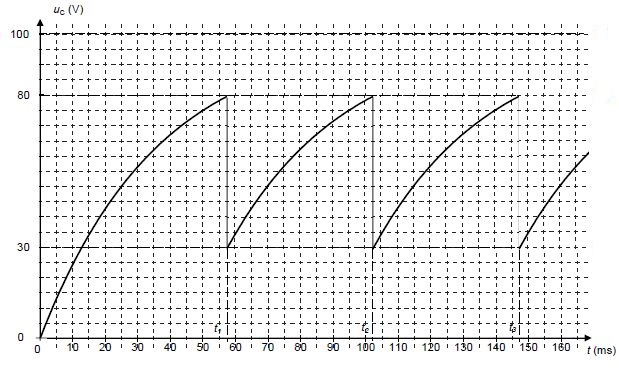
\includegraphics[width=0.65\linewidth]{elec/neon.jpg}
    \caption{Tension au bornes du néon $u_\textsc{c}$ en fonction du temps.}
\end{figure}

\`A $t<0$, le condensateur $C$ est déchargé et le tube est éteint. On allume le générateur à $t=0$.

Le circuit électrique, dans lequel est inséré le tube fluorescent, est schématisé ci-dessous :
\begin{circuit}[Modélisation du tube néon.]
      \draw (0,0)
      to [vsource, v^>=$E$] (0,3)
      to [R, l=$R$] (2,3)
      to [C, l_=$C$, *-*] (2,0)
      to [short] (0,0) {}
      (2,3) to [short] (4,3)
      to [nos, l^=$K$] (4,2)
      to [R, l^=$r$] (4,0)
      to [short] (2,0) {}
      (2.7,0) [open, v_=$u_\textsc{c}$] to (2.7,3) {} ;
      \draw [red, dashed] (3.6,-0.2) rectangle(4.8,3.2) ;
      \node [red] at (4.2,3.5) {Tube néon};
\end{circuit}
Le tube fluorescent est modélisé comme une résistance faible $r$ et un interrupteur $K$ en série. L'interrupteur est ouvert lorsque le tube est éteint et fermé lorsque le tube est allumé.
% Le tube fluorescent est modélisé comme une résistance faible $r$ et un interrupteur $K$ qui s'ouvre et se ferme selon si le tube est allumé ou éteint.

\paragraph{Données :} $E = 100$ V, $R = 60$ k$\Omega$, $r = 10$ $\Omega$, $C = 600$ nF.


\begin{questions}
    \questioncours Condensateurs et dipôles à comportement capacitifs.
    
    \question Décrire le comportement global observé en Fig.~\arabic{exercise}.1 ci-dessus et donner les valeurs de $U_e$ et $U_a$.
    
    \uplevel{On étudie d'abord le circuit entre $t = 0$ et $t_1$.}
    
    \question Simplifier le circuit \arabic{exercise}.1 dans ce cas puis résoudre l'équation différentielle vérifiée par $i$ et $u_\textsc{c}$.
    \question Calculer le temps $t_1$ de l'allumage du néon. Par analogie, quel est le temps $\tau$ du cycle d'allumage du néon ?
    
    \uplevel{On étudie maintenant d'abord le circuit entre $t_1$ et $t_1 + \varepsilon$.}
     
    \question En remarquant que $R\gg r$, simplifier le circuit \arabic{exercise}.1 dans ce cas puis résoudre l'équation différentielle vérifiée par $i$ et $u_\textsc{c}$.
    \question Calculer le temps $t'$ de décharge du condensateur. Justifier que l'on peut négliger ce temps dans le cycle du néon. Voit-on le néon s'allumer et s'éteindre ?
    
\end{questions}
\end{exercise}